%---------------------------------------------------------------------------------------------------
% GAME LOGIC
%---------------------------------------------------------------------------------------------------
\subsection{Bibliothèque \texttt{\gls{game_logic}}}
Dans le chapitre \ref{subsection_architecture_generale} nous avions introduit le module conceptuelle \og Rule Book \fg{}, qui génère un ensemble de pairs coup possible et plateau conséquence. Pour ce faire ce module doit pouvoir décider de la légalité d'un coup et de connaître ses conséquences. 

Nous avions également parlé dans le chapitre \ref{section_analyse_environnement} d'un agent \og Arbitre \fg{} maître du jeu qui a besoin d'un ensemble de règles à fin d'initialiser le plateau et d'appliquer ou de refuser les coups respectivement légaux et illégaux.

Il est claire que ces deux objets partagent un même ensemble de fonctions et de structures, donc une bibliothèque que nous appèlerons \texttt{game\_logic}  :
\begin{figure}[H] 
\centering
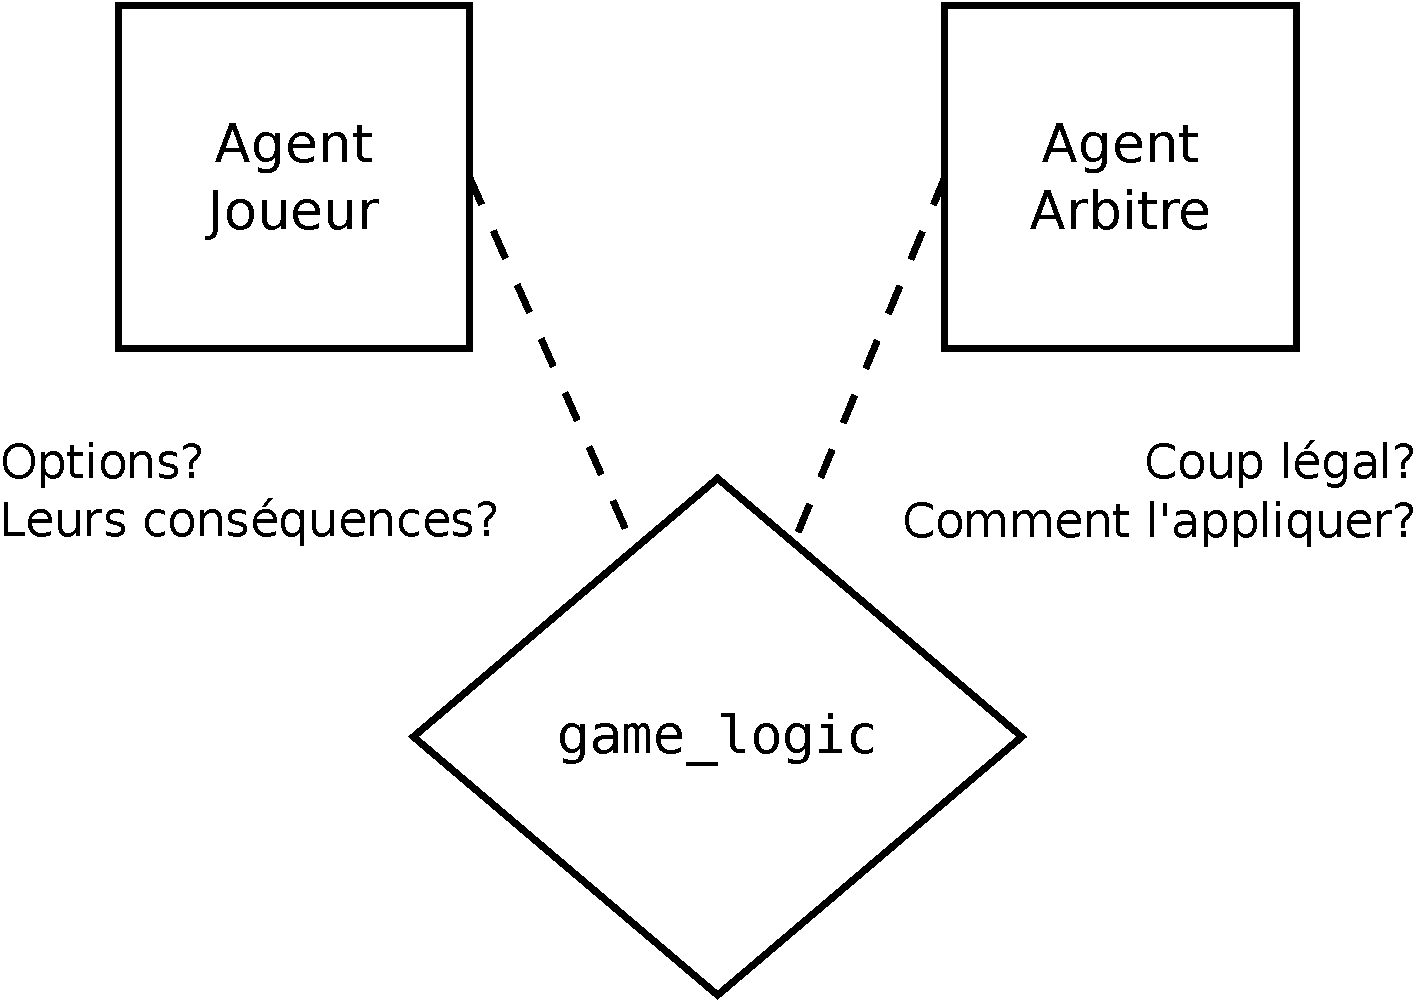
\includegraphics[width=\textwidth]{files/env/game_logic_shared} 
\caption{Partage de la bibliothèque \texttt{game\_logic}} 
\label{game_logic_shared}
\end{figure}
Précisement cette bibliothèque contient trois classes principales :
\begin{itemize}
\item \texttt{BoardMatrix} : Plateau sous forme matricielle avec accesseurs adaptés.
\item \texttt{Rules} : Interface implémenté par chaque jeu. Ses méthodes permettent de connaître :
\begin{itemize}
\item La forme du plateau et sa configuration initiale.
\item Qui joue en premier.
\item Quand la partie est gagné ou perdu et par qui, quand le match est nul.
\item Les coups possibles pour un joueur donnée.
\end{itemize}
\item \texttt{Game} : Associe un \texttt{Rules}, un \texttt{BoardMatrix}, un état et un joueur courant.
\end{itemize}
\begin{figure}[H] 
\centering
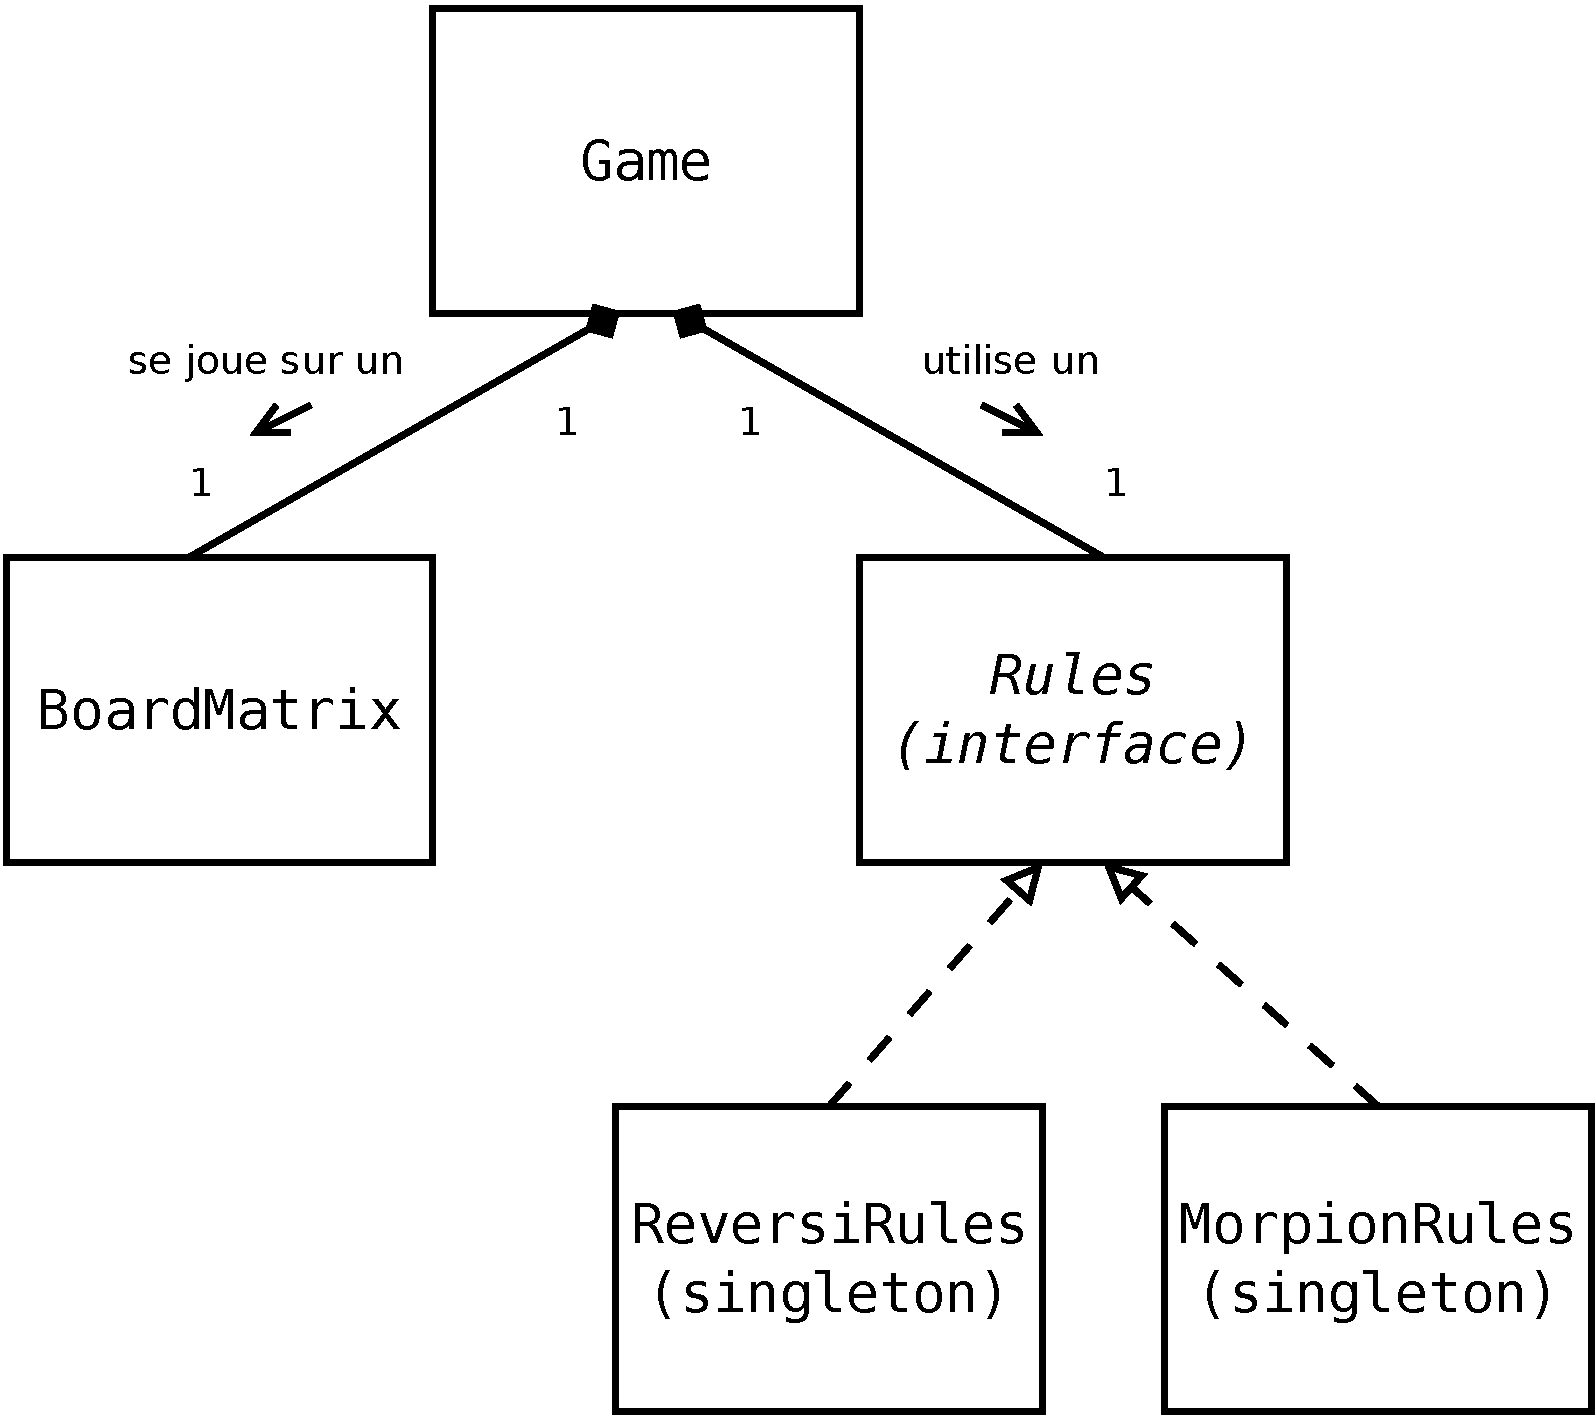
\includegraphics[width=\textwidth]{files/env/game_logic} 
\caption{Classes de la bibliothèque \texttt{game\_logic}} 
\label{game_logic}
\end{figure}

%---------------------------------------------------------------------------------------------------
% GAME SERVICE
%---------------------------------------------------------------------------------------------------
\subsection{Serveur \texttt{game\_service}}
Le chapitre \ref{section_analyse_environnement} conclut en proposant le modèle client-serveur pour les communications entre l'\emph{agent-joueur} et l'\emph{agent-arbitre}. L'arbitre et l'environnement, c'est à dire l'état du jeu, seront hébergés dans une application à part entière: un \og web service \fg{} appelé \texttt{game\_service}.
\subsubsection{Transfert des percepts}
Le client-joueur a tout d'abord besoin de percevoir son environnement, c'est à dire de connaître l'état courant du jeu. Ceci est envoyé par le serveur sous forme d'un  document \texttt{XML}\footnote{ XML : Extensible markup language. } grâce au protocole \texttt{HTTP}\footnote{ HTTP : Hyper-text transfer  protocol. }. Pilier du web, l'\texttt{HTTP} a l'avantage d'être très  répandu, ubiquité qui assure l'existence de bibliothèques ouvertes,  complètes, bien documentés et simples d'utilisation pour tout langage et  plateforme. Étant donnée que le développement du serveur ait débuté avant le reste du système, ce choix nous permettait d'éviter de se retrouver avec trop  de contraintes par la suite.
\subsubsection{Transfert des action}
Le client a également besoin d'envoyer ses coups au serveur. Pour ceci il suffit d'utiliser un paramétrage de la requête pour indiquer :
\begin{itemize}
\item celui qui joue,
\item une ligne,
\item une colonne.
\end{itemize}
Il nous est désormais possible d'interagir avec le serveur en écrivant manuellement nos coups dans la barre d'adresse et en lisant le document XML renvoié. Cette manière de jouer est peu ergonomique, mais elle nous a permi de tester le fonctionnement du serveur en son intégralité bien avant la construction d'une interface graphique.

À noter également, vu qu'il n'y a pas d'authentification ou de suivi des clients, qu'il est possible de \og tricher \fg{} en prenant le tour de l'autre joueur  : nous supposons ici qu'il n'y a simplement pas de félons. Par la suite identificateur de session, dans un cookie par exemple, pourrait empêcher ce genre d'abus. 
\subsubsection{Constitution des réponses}
Pour analyser toutes ces requêtes paramétrés et composer une réponse la technologie \og Java Servlet \fg {} est utilisé. Une classe Java est instancié par notre serveur Tomcat pour traiter une seule requête : l'objet est détruit immédiatement après avoir envoyé sa réponse, dans ce cas sous forme d'un document XML.

Cette technologie orienté prototypage rapide est très simple à utiliser mais nous permet pourtant de gérer de multiples requêtes concurrentes, donc de faire tourner un très grand nombre de jeux entre différentes paires de clients. Il suffit d'ajouter un paramètre de plus à la requête pour préciser l'identificateur du jeu, et un singleton côté serveur pour stoquer les jeux et gérer les accès concurrents.
\subsubsection{Conclusion}
Le serveur correspond finalement un \og Service Web \fg{}, c'est à dire un programme fournissant des données destinés à etre lus par des autres programmes et non des humains :
\begin{figure}[H] 
\centering
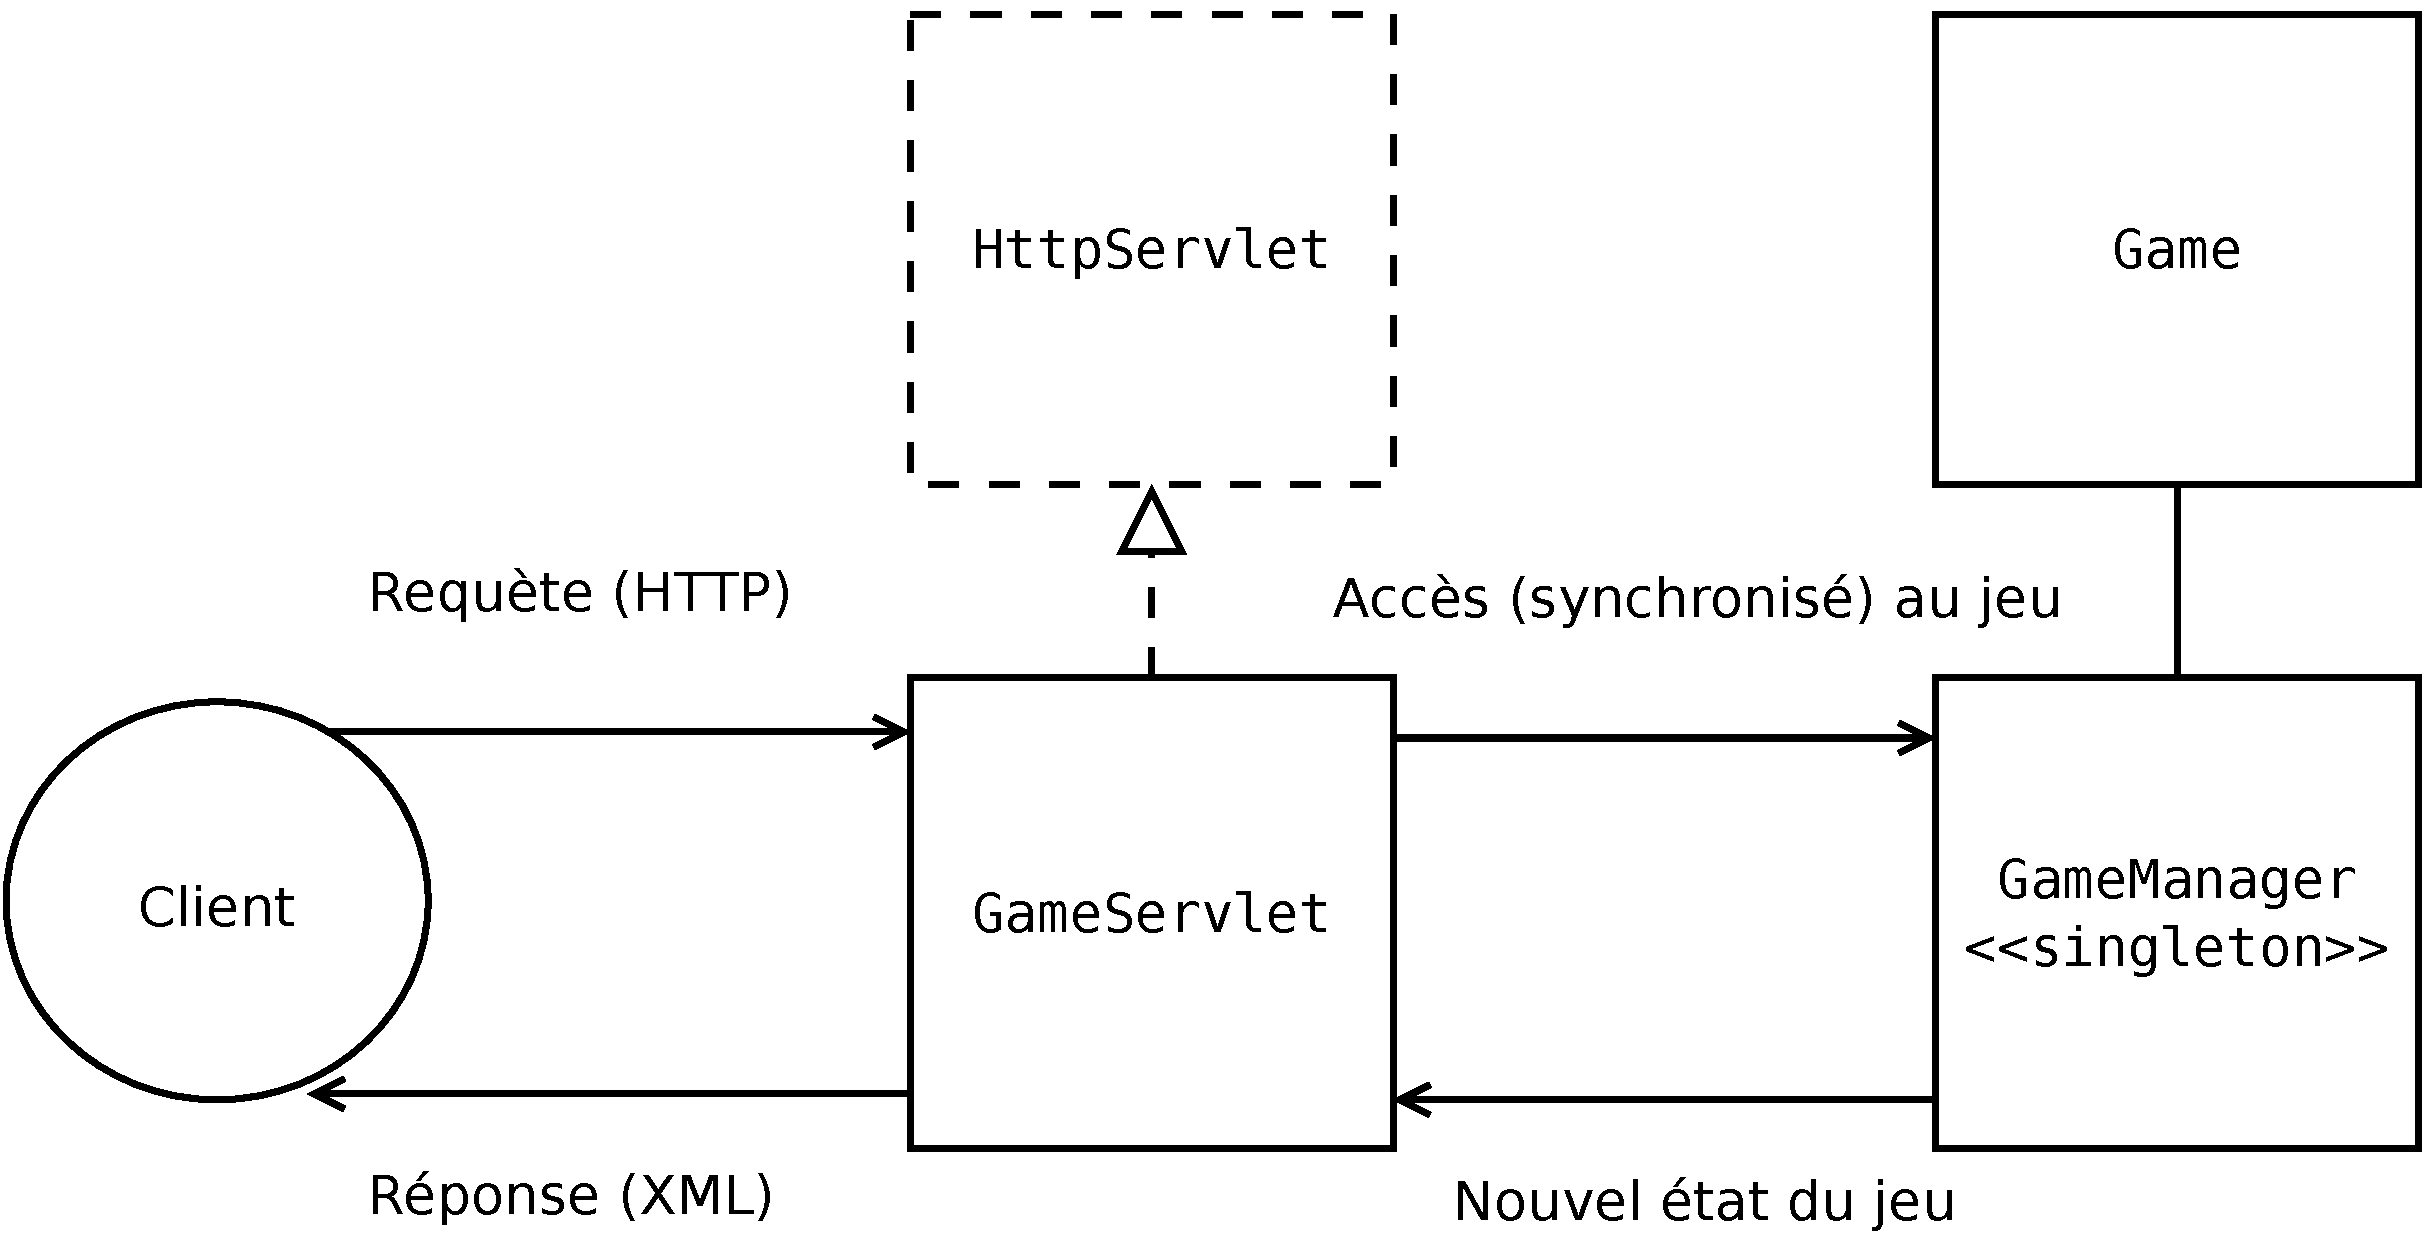
\includegraphics[width=\textwidth]{files/env/game_service} 
\caption{Classes du Service Web \texttt{game\_service}} 
\label{game_service}
\end{figure}
Ici le \texttt{GameManager} sert de base de données temporaire : c'est un conteneur de \texttt{Game}, classe de la bibliothèque \texttt{game\_logic} que nous venons d'introduire. Chaque \texttt{Game} possédant une réference vers un \texttt{Rules} il est possible pour le serveur d'arbitrer tous les parties simultanément.

%---------------------------------------------------------------------------------------------------
% CLIENT HUMAIN
%---------------------------------------------------------------------------------------------------
\subsection{Client humain}

%---------------------------------------------------------------------------------------------------
% CLIENT MACHINE
%---------------------------------------------------------------------------------------------------
\subsection{Client machine}